\section{Bagian III --- Pembuktian Teoretis dan Empiris Batasan MLP Classifier untuk Image Generation}

\subsection{Uraian matematis}
\textbf{(1) $P(y\mid x)$ berbanding $P(x)$.} Cross-Entropy hanya memaksimalkan $\log p(y|x)$; tidak ada suku yang
menghukum hilangnya informasi tentang $x$ selama label tetap dapat ditebak. Pada rantai Markov
$y\to x\to z_{\text{MLP}}\to\hat{y}$, \emph{data processing inequality} memberi $I(x;z)\le H(x)$ dan
optimum klasifikasi hanya menuntut $I(z;y)=I(x;y)\le H(y)=\log 10\approx 3{,}32$ bit. Representasi minimal-cukup
(\emph{information bottleneck}, $\min I(x;z)-\beta I(z;y)$) karenanya membuang variasi intra-kelas (pose, tekstur, ukuran)
yang justru dibutuhkan untuk merekonstruksi atau mensintesis $x$. Model generatif sebaliknya memodelkan
$p(x)=\int p(x|z)p(z)\,dz$ sehingga \emph{seluruh} variasi $x$ harus terkode.

\textbf{(2) $W^{\top}\neq W^{-1}$ dan ReLU tidak injektif.} $W_1\in\mathbb{R}^{256\times784}$ berrank paling tinggi 256, sehingga
menurut teorema rank--nullity terdapat ruang nol berdimensi $784-256=528$: setiap $x+v$ dengan $v\in\ker W_1$
menghasilkan pra-aktivasi yang sama dan tidak dapat dibedakan. Invers kiri tidak ada; transpos hanya sama dengan invers
bila $W^{\top}W=I$ (kolom ortonormal), padahal bobot terlatih memiliki
$\lVert W_1^{\top}W_1-I\rVert_F/\lVert I\rVert_F=\WoneOrth$ dengan bilangan kondisi \WoneCond. ReLU$(u)=\max(0,u)$ memetakan seluruh
setengah-ruang $u<0$ ke 0; pada test set \ReluOne\ pra-aktivasi lapisan 1 dan \ReluTwo\ lapisan 2 terpotong secara ireversibel.
Akibatnya $W^{\top}$ hanya menghasilkan \emph{superposisi template} baris bobot, bukan citra.

\textbf{(3) Tanpa regularisasi kerapatan $P(z)$.} Tidak ada suku seperti $D_{\text{KL}}(q(z|x)\Vert p(z))$ sehingga
distribusi $z_{\text{MLP}}$ bebas berbentuk apa pun (berkelompok per kelas, \ZeroFrac\ komponennya bernilai nol eksak).
Gaussian diagonal $\mathcal{N}(\mu_z,\mathrm{diag}\,\sigma_z^2)$ tidak menutupi manifold ini: \NegFrac\ komponen sampel
bernilai negatif---nilai yang mustahil dihasilkan ReLU.

\subsection{Hasil eksperimen Tahap 1--5}
\textbf{Tahap 1.} MLP $784\!\to\!256\!\to\!64\!\to\!10$ dilatih 25 epoch (checkpoint terbaik dipilih dari akurasi
validation) dan mencapai \textbf{akurasi test \MLPacc\%} ($\ge$ 88\%). Bobot $W_1,W_2,W_3$ dan $z_{\text{MLP}}$ disimpan.

\begin{table}[h]
\centering\small
\caption{Ringkasan kuantitatif eksperimen batasan MLP Classifier (Test Set, 7.000 citra).}
\label{tab:mlp}
\begin{tabular}{@{}lccccl@{}}
\toprule
Eksperimen & MSE $\downarrow$ & PSNR (dB) $\uparrow$ & SSIM $\uparrow$ & Var. intra-kelas & Keterangan \\
\midrule
T2: $W^{\top}$ dari one-hot $y_c$ (vs citra rata-rata kelas) & \TtwoMSE & \TtwoPSNR & \TtwoSSIM & -- & bercak kabur \\
T3: $W^{\top}$ dari $z_{\text{MLP}}$ & \TthreeMSE & \TthreePSNR & \TthreeSSIM & -- & tidak mirip citra \\
T3: pseudo-invers $W^{+}$ dari $z_{\text{MLP}}$ & \TpinvMSE & \TpinvPSNR & \TpinvSSIM & -- & tetap gagal \\
T4: Frozen decoder dari $z_{\text{MLP}}$ & \FdMSE & \FdPSNR & \FdSSIM & \FdVar & detail hilang \\
T4: Vanilla AE ($z_{\text{AE}}\in\mathbb{R}^{64}$) & \AeMSE & \AePSNR & \AeSSIM & \AeVar & pembanding \\
\bottomrule
\end{tabular}
\end{table}

\textbf{Tahap 2 (transpos dari vektor kelas).} $\hat{x}=\mathrm{Sigmoid}(W_1^{\top}\mathrm{ReLU}(W_2^{\top}\mathrm{ReLU}(W_3^{\top}y_c)))$
menghasilkan pola bercak bertekstur frekuensi tinggi (Gambar~\ref{fig:mlp}, baris 2a). Terhadap citra rata-rata
tiap kelas, SSIM hanya \TtwoSSIM: siluet kelas tidak muncul karena tiap baris $W_1$ adalah \emph{detektor} fitur
diskriminatif (positif dan negatif bercampur), bukan potongan citra.

\textbf{Tahap 3 (transpos dari fitur laten citra uji).} Proyeksi $\mathrm{Sigmoid}(W_1^{\top}\mathrm{ReLU}(W_2^{\top}z_{\text{MLP}}))$
menghasilkan SSIM \TthreeSSIM\ terhadap citra asli. Bahkan pseudo-invers Moore--Penrose $W^{+}$, yang merupakan
solusi kuadrat-terkecil terbaik untuk sistem linear, hanya mencapai SSIM \TpinvSSIM: informasi yang telah dibuang oleh ReLU
dan oleh proyeksi ke ruang berdimensi 64 tidak dapat dipulihkan oleh operasi linear apa pun.

\textbf{Tahap 4 (frozen latent decoding).} Dengan seluruh bobot MLP dibekukan (\texttt{requires\_grad=False}),
decoder $64\!\to\!256\!\to\!784$ yang dilatih 30 epoch dengan MSE (arsitektur dan jumlah epoch identik dengan decoder Vanilla AE)
hanya mencapai PSNR \FdPSNR\ dB dibanding \AePSNR\ dB pada Vanilla AE (MSE \FdAeRatio$\times$ lebih besar).
Rasio varians intra-kelas rekonstruksi terhadap citra asli turun dari \AeVar\ (AE) menjadi \FdVar: decoder hanya
dapat menghasilkan ``prototipe kelas'' karena variasi di dalam kelas sudah tidak ada di $z_{\text{MLP}}$.
Menariknya, akurasi MLP pada rekonstruksi frozen decoder (\FdAcc\%) setara dengan rekonstruksi AE (\AeAcc\%): informasi
\emph{kelas} terjaga sempurna, sedangkan informasi \emph{citra} hilang---bukti langsung efek information bottleneck.

\textbf{Tahap 5 (sampling dari ruang laten MLP).} 2.000 sampel $z_{\text{rand}}\sim\mathcal{N}(\mu_z,\mathrm{diag}\,\sigma_z^2)$
diteruskan ke decoder Tahap 4. Jarak rata-rata sampel ke kode training terdekat adalah \NNrand, sedangkan kode test riil
hanya \NNreal\ (\NNratio$\times$ lebih jauh): sampel jatuh di wilayah kosong. Hasilnya berupa citra kabur campuran
beberapa kelas (Gambar~\ref{fig:mlp}, baris 4); entropi prediksi MLP pada sampel ini \EntMLP\ nat, lebih tinggi daripada
sampel VAE (\EntVAE) dan citra riil (\EntReal), serta distribusi kelasnya timpang (kelas Trouser hanya \TrouserMLP\ dari 2.000).
FID sampel ini adalah \FIDmlp, jauh di atas VAE (\FIDvae).

\begin{figure}[h]
\centering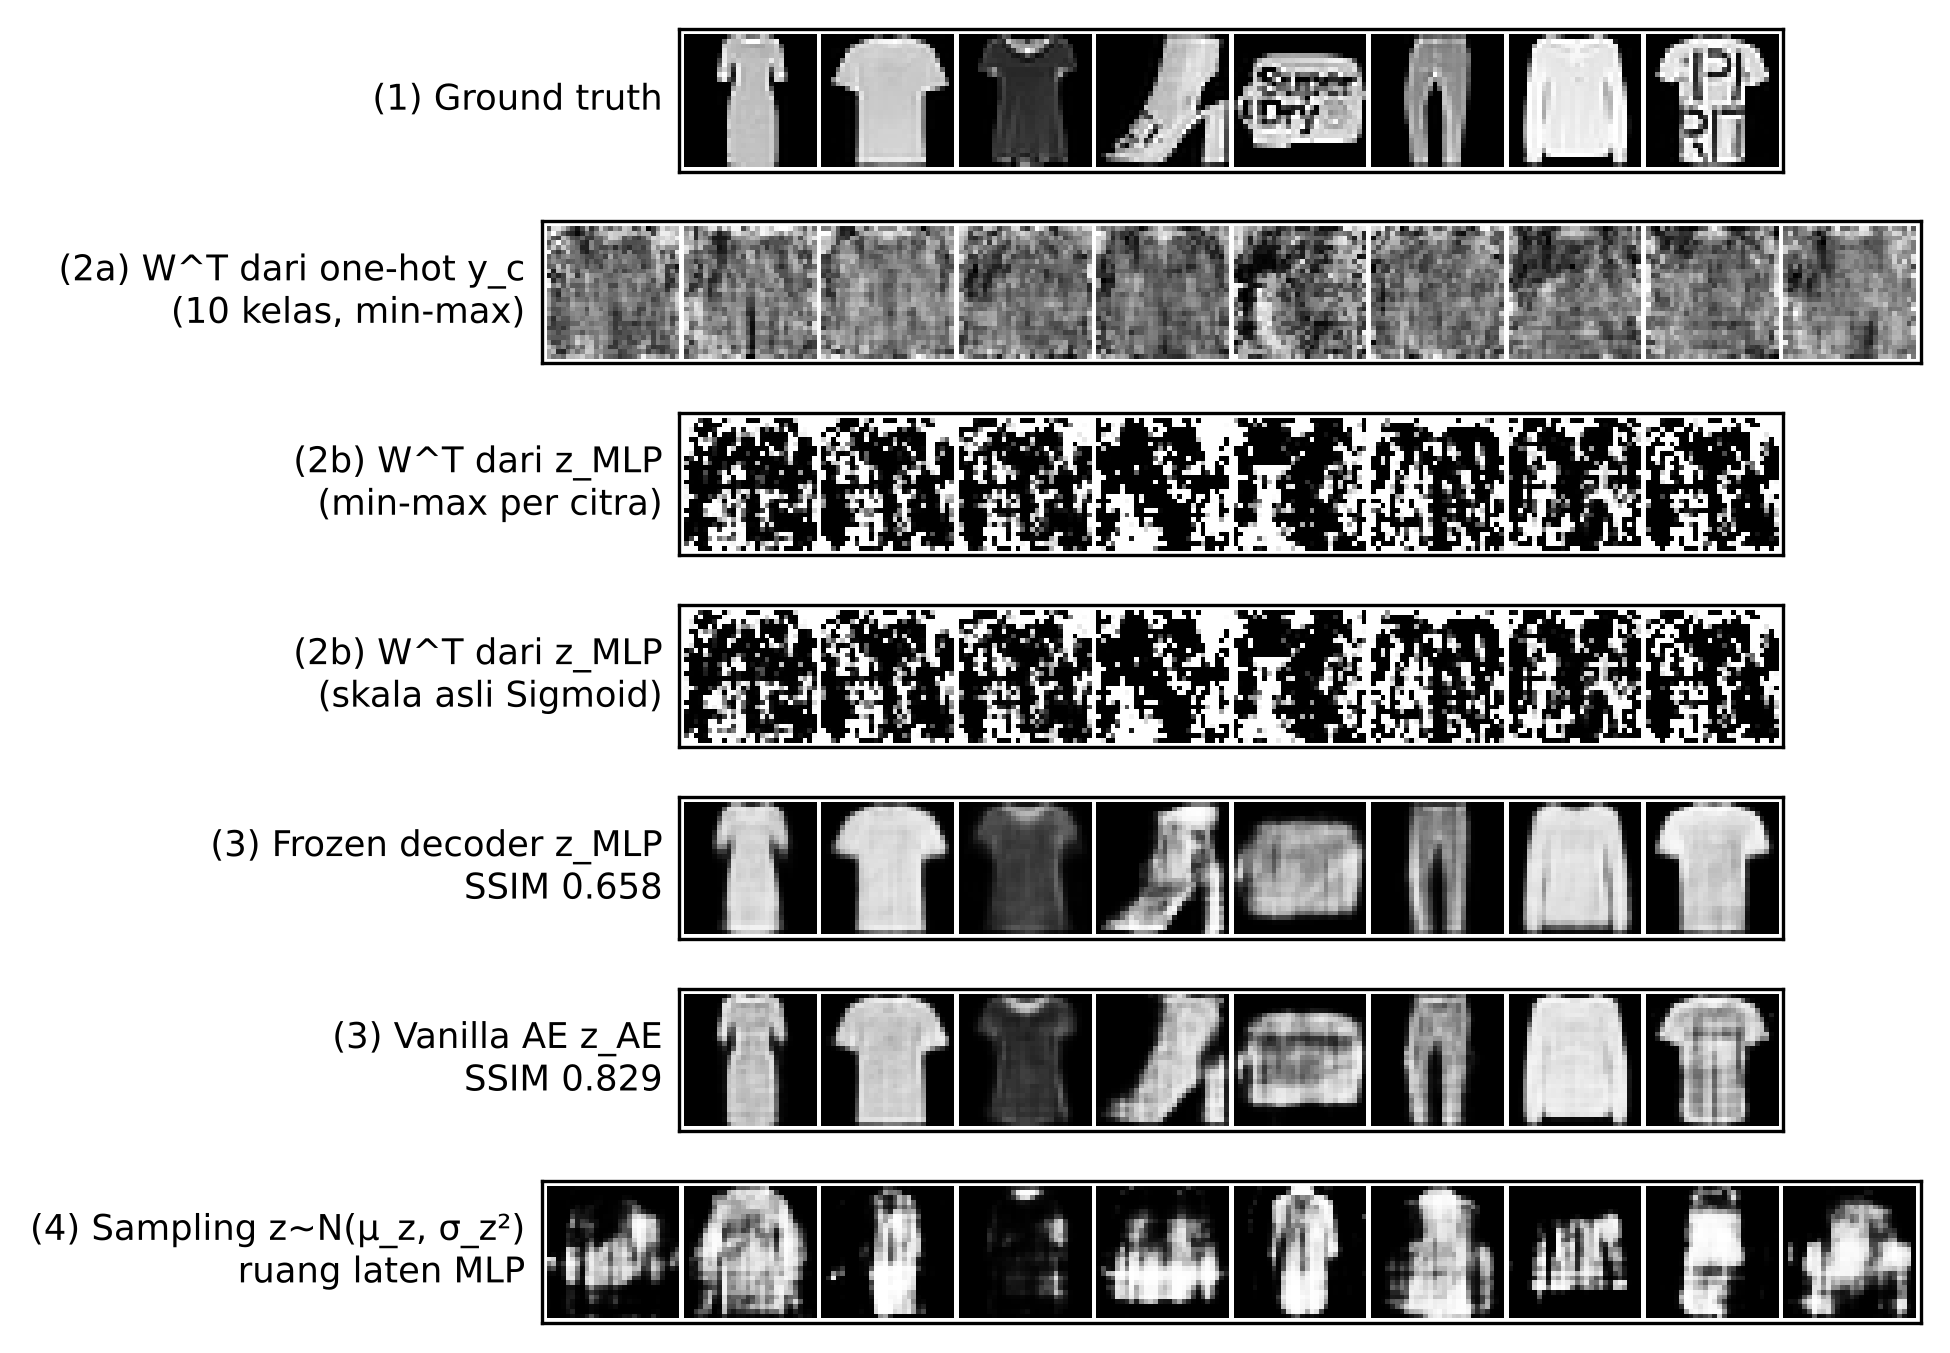
\includegraphics[width=0.92\linewidth]{../outputs/figures/fig3_mlp_batasan.png}
\caption{\textbf{Figur 3.} Bukti empiris batasan MLP Classifier: (1) ground truth; (2a) proyeksi balik $W^{\top}$ dari
one-hot 10 kelas (urutan T-shirt$\to$Ankle boot); (2b) proyeksi balik $W^{\top}$ dari $z_{\text{MLP}}$ (dinormalisasi min-max agar
pola terlihat, lalu dalam skala asli); (3) frozen latent decoder vs Vanilla AE; (4) random prior sampling pada ruang laten MLP.}
\label{fig:mlp}
\end{figure}
